\clearpage
\section{Modelarea sistemului informațional}

\subsection{Book Mall}

În cadrul acestui proiect a fost analizat și modelat un sistem de gestiune a
librării online, numele acestui sistem va fi Book Mall. Acest sistem va fi o
aplicație web, accesibil din browser pe orice paltformă. Pentru început va
oferi cărți electronice în format pdf apoi cu timpul va fi adăugat suportul
pentru alte formate și convertirea pe server a fișierelor.

Printre cele mai populare sisteme care oferă un funcțional asemănător sunt:
\begin{itemize}
    \item amazon;
    \item apple Books;
    \item eBooks.com;
    \item smashwords;
    \item barnes and Noble;
    \item kobo;
    \item google Play Books;
    \item harlequin.
\end{itemize}
Prețul pe aceste paltforme la cărțile electronice în unele cazuri este mai mare ca a cărților fizice, de aceia acest sistem are ca scop să ofere prețuri rezonabile.

Scopul acestui proiect este modelarea sistemului unei librării online cu funcțional de bază, cu posibilitatea de îmbunătățire în viitor. Funcționalul dorit este autentificarea, gestionarea utilizatorilor și a cărților, căutarea și descărcarea cărților.

\subsection{PlantUML}
Pentru modelarea acestui sistem va fi utilizat PlantUML\cite{PlantUML}. Motivul utilizării
acestui software este faptul că permite utilizatorilor să creeze diagrame
dintr-un limaj de text simplu și licența open-source. Faptul că utilizează un
un fișer text permite concentrarea asupra modelării ci nu asupra aspectului
vizual și amplasării a elementelor grafice. Imaginile pot fi transmise ca PNG,
SVG, Latex și chiar ASCII Art. Plantuml de asemenea poate fi utilizat pentru a
permite oamenilor nevăzători să proiecteze și să citească diagramele UML.

Fiind că diagramele sunt scrise într-un fișier text, poate fi utilizat orice
editor de text, în cazul acestui proiect a fost utilizat Neovim\cite{Neovim}.

\newpage
\subsection{Diagrama cazului de utilizare}

Pentru ca librăria să poată funcționa fară probleme este nevoie ca
administratorii să urmărească respectarea regulilor de utilizare a sistemului
și să eleveze utlizatorii la rolul de autor în cazul în care aceștia doresc să
încarce cărți. În figura \ref{fig:usecase0} poate fi observată interacțiunea
administratorului cu sistema acesta având posibilitatea de a se autentifica,
gestiona cărți, gestiona abonamente, șterge utilizatori, căuta cărți și
descărca cărți. Un rol important al administratorului este de a gestiona
abonamente și șterge utilizatori alți utilizatori nefind capabili să facă
aceste acțiuni. Utilizatorii nu se pot înregistra ca administratori acest, acest
rol poate fi alocat prin manipularea directă a bazei de date.
\begin{figure}[H]
    \begin{center}
        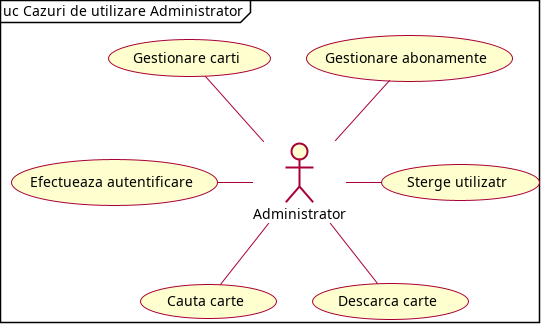
\includegraphics[width=12cm]{figures/usecase/usecase.png}
        \caption{Interacțiunea Administratorului cu interfața}
        \label{fig:usecase0}
    \end{center}
\end{figure}

Autorul sau moderatorul este actorul care spre deosebire de utilizatorul simplu
poate încărca cărți și este recomandat ca aceste cărți să îi aparțină. În
figura \ref{fig:usecase1} se observă interacțiunea Autorului cu sistema la fel
ca administratorul, autorul poate să se autentifice, să gestioneze carți însă
doar care ii aparțin, să caute cărți și să descarce cărți, el nu poate să
gestioneze abonamentele și nici să șteargă utilizatori. Pentru ca un utilizator
să obțină acest rol este nevoie ca un administrator să îl eleveze.
\begin{figure}[H]
    \begin{center}
        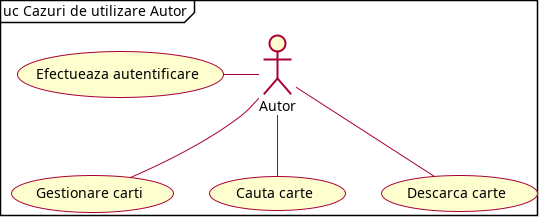
\includegraphics[width=13cm]{figures/usecase/usecase_001.png}
        \caption{Interacțiunea Autorului cu interfața}
        \label{fig:usecase1}
    \end{center}
\end{figure}

Utilizatorul este cel mai de bază actor al sistemului respectiv, și se referă
la un utilizator înregistrat, acest rol este dat implicit la înregistrarea în
sistemă. În figura \ref{fig:usecase2} se observă interacțiunea Utilizatorului
cu sistema. Utilizatorul are posibilitatea de a se autentifica de a descărca și
căuta cărți.
\begin{figure}[H]
    \begin{center}
        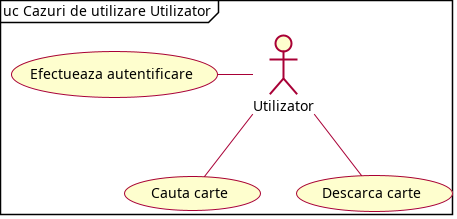
\includegraphics[width=10cm]{figures/usecase/usecase_002.png}
        \caption{Interacțiunea Utilizatorului cu interfața}
        \label{fig:usecase2}
    \end{center}
\end{figure}

În figura \ref{fig:usecase3} se descrie mai detaliat posibilitatea de
gestionarea carți. După cum se poate observa există posibilitatea de a încărca,
modifica și șterge cărți. Totodată pentru fiecare caz este necesar de verificat
permisiuni, astfel autorii își pot modifica doar cărțile lor iar utilizatorii
simpli nu au acces la acest funcțional.
\begin{figure}[H]
    \begin{center}
        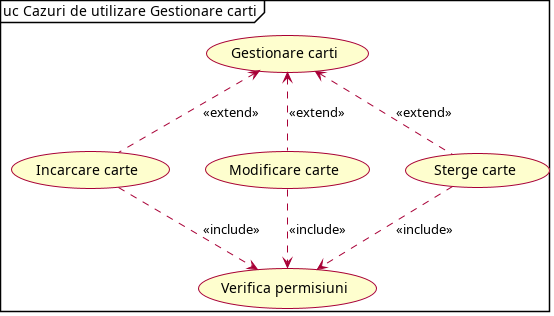
\includegraphics[width=14cm]{figures/usecase/usecase_003.png}
        \caption{Gestionare cărți}
        \label{fig:usecase3}
    \end{center}
\end{figure}

În figura \ref{fig:usecase4} este descrisă autentificarea. Actorii au
posibilitatea de a se înregistra cu rolul de utilizator și odată ce au un cont
pot să se logheze utilizând datele credențiale. În cazul în care actorul și-a
uitat parola el poate să o reseteze utilizând adresa de email.
\begin{figure}[H]
    \begin{center}
        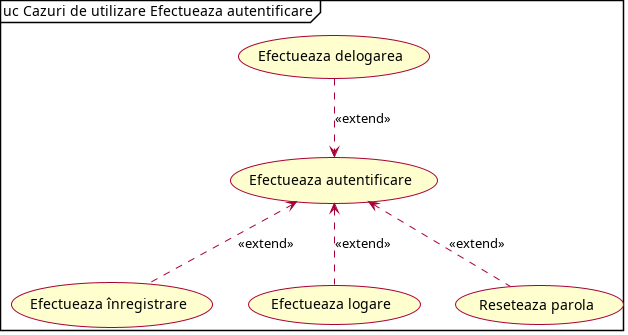
\includegraphics[width=13cm]{figures/usecase/usecase_004.png}
        \caption{Autentificare}
        \label{fig:usecase4}
    \end{center}
\end{figure}

Descărcarea cărților este descrisă în figura \ref{fig:usecase5}.
Este necesar ca utilizatorul să fie autentificat și să dețină cartea respectivă
pentru a o putea descărca, în cazul în care el nu deține cartea poate să o
cumpere și mai apoi să o descarce.
\begin{figure}[H]
    \begin{center}
        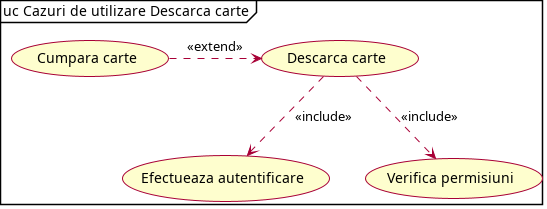
\includegraphics[width=14cm]{figures/usecase/usecase_005.png}
        \caption{Descarcare carte}
        \label{fig:usecase5}
    \end{center}
\end{figure}

\newpage
\subsection{Diagrama secvență}

În diagrama din figura \ref{fig:sequence0} este reprodus procesul ștergere a
unui utilizator. Acest proces decurge în 12 pași. În primul rând este nevoie ca
administratorul să obțină lista tuturor utilizatorilor apoi poate selecta acest
utilizator după ID și să îl șteargă.

Diagrama de secvență, figura \ref{fig:sequence1} pentru cazul de utilizare
gestionare cărți decurge în 22 de pași. Autorul introduce documentul unei cărți
și datele despre aceasta (titlul, autorul, ect.) apoi apasă butonul de creare
și informația este transmisă către server. Un răspuns este afișat ca rezultat.
Autorul poate selecta o carte și să o șteargă sau modifice.

În figura \ref{fig:sequence2} putem observa descărcarea cărții, această
diagramă decurge în 26 de pași. Utilizatorul are posibilitatea de a căuta o
carte după titlu și să acceseze pagina cărții care îl interesează. Utilizatorul
poate procura cartea respectivă sau să o descarce în caz că deja a cumpărato.

\begin{figure}[H]
    \begin{center}
        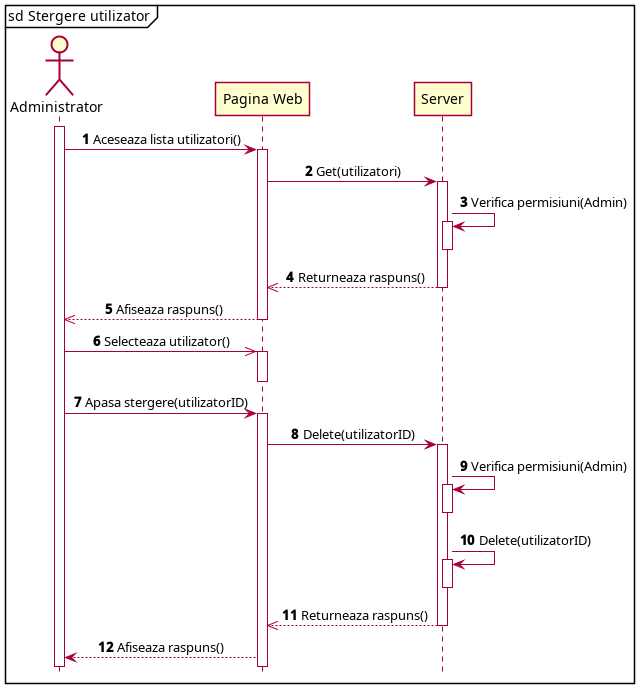
\includegraphics[width=15cm]{figures/sequence/sequence.png}
        \caption{Ștergerea utilizator}
        \label{fig:sequence0}
    \end{center}
\end{figure}

\begin{figure}[H]
    \begin{center}
        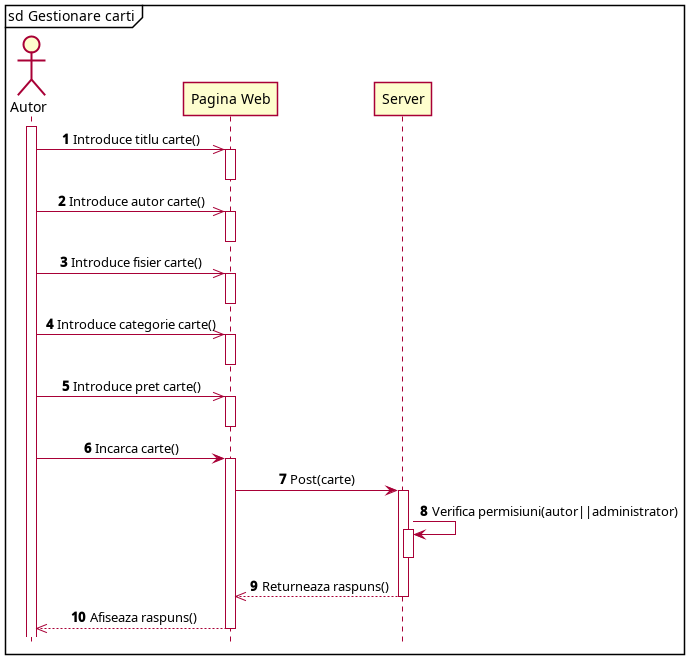
\includegraphics[width=15cm]{figures/sequence/sequence_001.png}
        \caption{Gestionare cărți}
        \label{fig:sequence1}
    \end{center}
\end{figure}

\begin{figure}[H]
    \begin{center}
        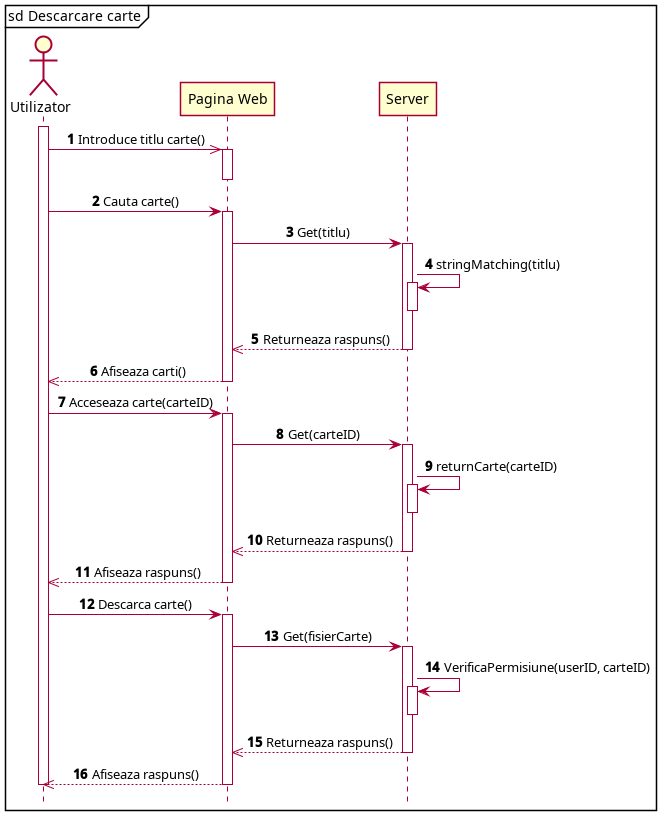
\includegraphics[width=15cm]{figures/sequence/sequence_002.png}
        \caption{Descărcare carte}
        \label{fig:sequence2}
    \end{center}
\end{figure}

\newpage
\subsection{Diagrama de colaborare}

În figura \ref{fig:collaboration} este prezentată interacțiunea obiectelor în
procesul de gestionare a cartilor. Autorul poate trimite mesaj de introducere,
modificare sau stergere a unei cărți, pagina va trimite datele către controler
pentru a le verifica iar apoi controlerul va apela metode din BuisnessLogic
pentru a actualiza informația despre carte.
\begin{figure}[H]
    \begin{center}
        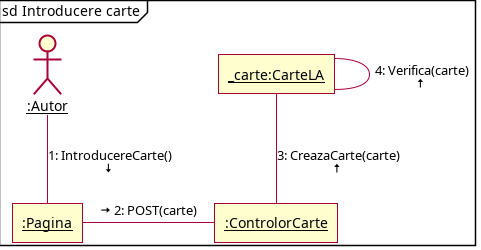
\includegraphics[width=12cm]{figures/collaboration/collaboration.png}
        \caption{Gestionare carte}
        \label{fig:collaboration}
    \end{center}
\end{figure}

\newpage
\subsection{Diagramă de clasă}

Figura \ref{fig:class0} conține mai multe clase și relațiile dintre acestea.
Utilizatorul este clasa de bază pentru actorii Client, Autor și Administrator.
Cele mai multe atribue și metode pentru actori sunt definite în clasa
Utilizator iar clasele care moștenes doar unele variații.
\begin{figure}[H]
    \begin{center}
        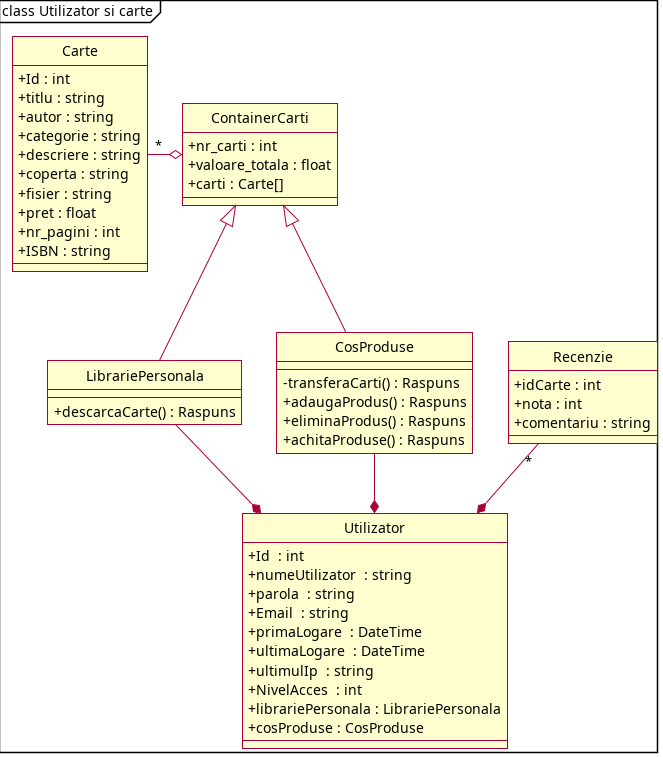
\includegraphics[width=15cm]{figures/class/class.png}
        \caption{Reprezentarea actorilor cu diagrama de clasă}
        \label{fig:class0}
    \end{center}
\end{figure}

\newpage
În figura \ref{fig:class1} se trage atenția asupra clasei Carte și rolul
acesteia în sistem. Utilizatorii conțin o singura  Librărie Personală și un
singur Coș de Produse care sunt containere de cărți. Un container de cărți
poate conține mai multe cărți.
\begin{figure}[H]
    \begin{center}
        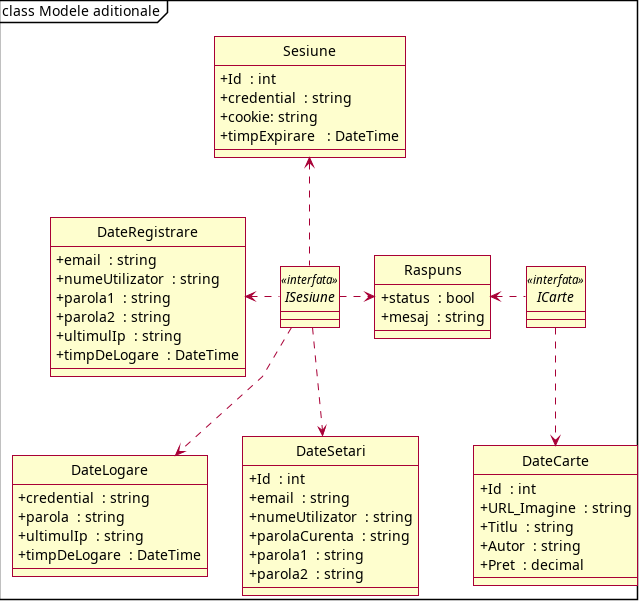
\includegraphics[width=15cm]{figures/class/class_001.png}
        \caption{Reprezentarea cărților cu diagrame de clasă}
        \label{fig:class1}
    \end{center}
\end{figure}

\newpage
\subsection{Diagrama de stare}
 
În figura \ref{fig:state0} putem observa stările prin care trece un obiect de
tipul SessionBL în procesul de logare al utilizatorului.
\begin{figure}[H]
    \begin{center}
        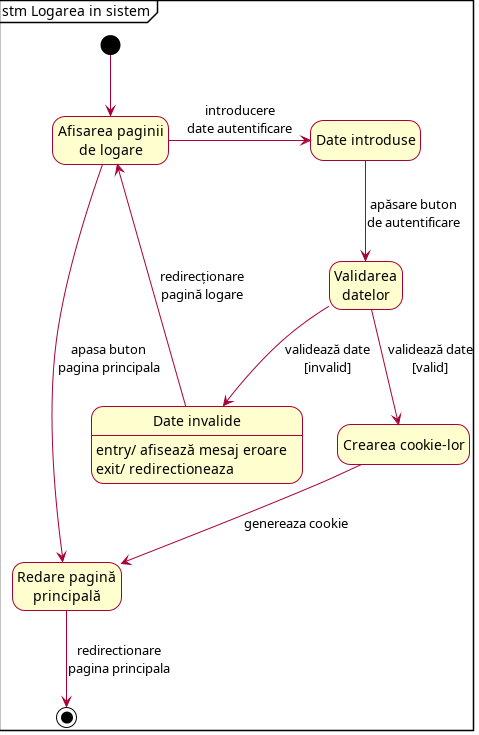
\includegraphics[width=15cm]{figures/state/state.png}
        \caption{Logarea în sistemă}
        \label{fig:state0}
    \end{center}
\end{figure}

\newpage
În figura \ref{fig:state1} putem observa stările prin care trece un obiect de tipul ProductBL în procesul de crearea a unui produs nou.
\begin{figure}[H]
    \begin{center}
        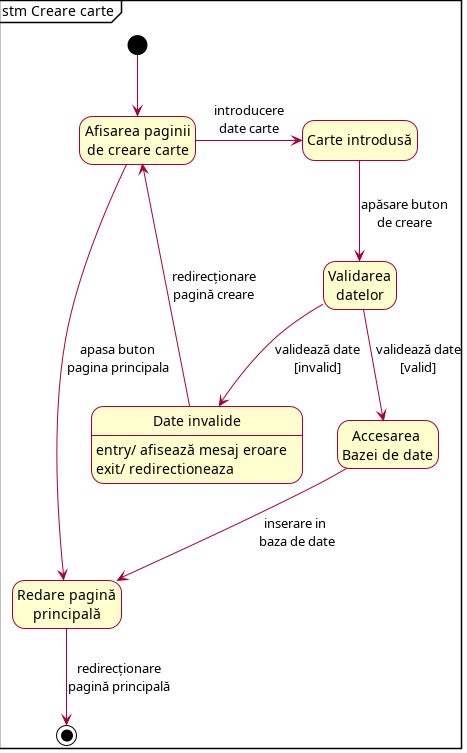
\includegraphics[width=15cm]{figures/state/state_001.png}
        \caption{Creare carte}
        \label{fig:state1}
    \end{center}
\end{figure}

\newpage
\subsection{Diagrama de activități}

În figura \label{fig:activity} vedem diagrama de activități pentru cazurile de
utilizare căutare și descărcare carte. În cazul în care cartea este disponibilă
însă nu ii aparține utilizatorul acesta poate să o cumpere și apoi să o
descarce.
\begin{figure}[H]
    \begin{center}
        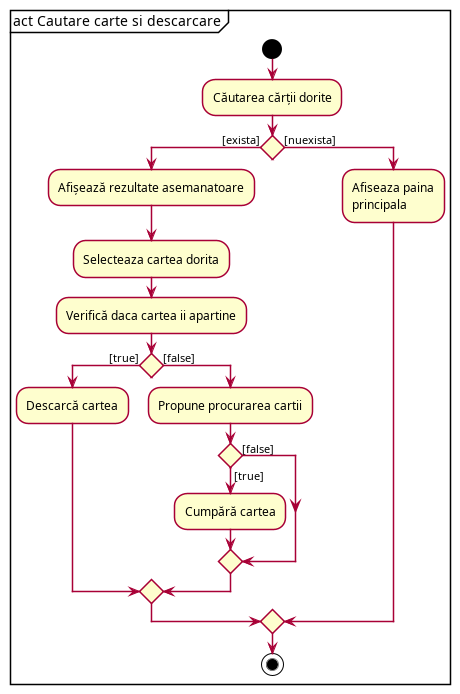
\includegraphics[width=10cm]{figures/activity/activity.png}
        \caption{Căutarea și desărcarea cărților}
        \label{fig:activity}
    \end{center}
\end{figure}

